\chapter{Feature-based approach}
\label{cha:FeatureApproach}

To solve the main drawbacks of finding reliable point correspondences between $C_1$ and $C_2$ another approach is drawn on the an initial alignment on point features. The approach is closely related to Mitra \cite{Mitra07} and only proposes slight deviations of the approach to be compared with the reference approach. The main part of the approach is the computation of point feature histograms, namely FPFH \cite{FPFH} as proposed by Mitra et al \cite{Mitra07}.

\section{FPFH}
\label{FPFH}
The ``Fast Point Feature histograms'' algorithm is implemented in 2D. It is an improved approach of the `'Persistent Point Feature Histogram for 3D Point Clouds'' \cite{PPFH}. The choice of those features are the following: 
%%
\begin{itemize}
	\item rotation- and scale-invariant features
	\item easy comparison of feature histograms
	\item straightforward implementation
	\item approval of approach
	\item easy adaption from different dimensions (2D and 3D)
\end{itemize}
%%
By using a histogram the neighborhoods' geometrical properties can be provided in form of the mean surface curvature at a point $\boldsymbol{p}$. 

\subsection{Normal estimation}

As a first step, the normals of all points from the input clusters $C_1$ and $C_2$ need to be estimated \cite{normals}. Those is achieved by taking all points $k$ within a radius $r$ from a point $\boldsymbol{p}$. Subsequently, a least error fit straight line $X$ in the form $ax + by +c = 0$ to all $k$ points is computed by minimizing the squared distances from all points $\boldsymbol{p_i(x_i,y_i)}$
%%
\begin{equation}
\begin{split}
dist^2(x_i, y_i) = (ax_i + by_i + c)^2
\\
e =   \displaystyle\sum_{i=1}^{k} dist^2(x_i, y_i)
\end{split}
\end{equation}
%%
to $X$. This is done by computing the unknown parameters $a, b$ of $X$ with the covariance matrix 
%%
\begin{equation}
\begin{pmatrix}
\overline{x^2} - \overline{x} \cdot \overline{x} & \overline{xy} -\overline{x} \cdot \overline{y}\\
\overline{xy} -\overline{y} \cdot \overline{x} & \overline{y^2} -\overline{y} \cdot \overline{y}
\end{pmatrix} \cdot \begin{pmatrix}
a \\
b
\end{pmatrix} = \lambda \cdot \begin{pmatrix}
a \\
b
\end{pmatrix}
\end{equation}
%%
resulting in two pairs of an eigenvalue and eigenvector $(n_1,\lambda_1)$ and $(n_2,\lambda_2)$. The normal of $\boldsymbol{p}$ is computed solving the linear equation for the normal vector $\vec{n_2}$ which is represented by $\lambda_2$. The procedure is conducted for all points from $C_1$ and $C_2$ (see figure \ref{fig:normalEstimation}). 
%%
\begin{figure}[H]
	\centering
	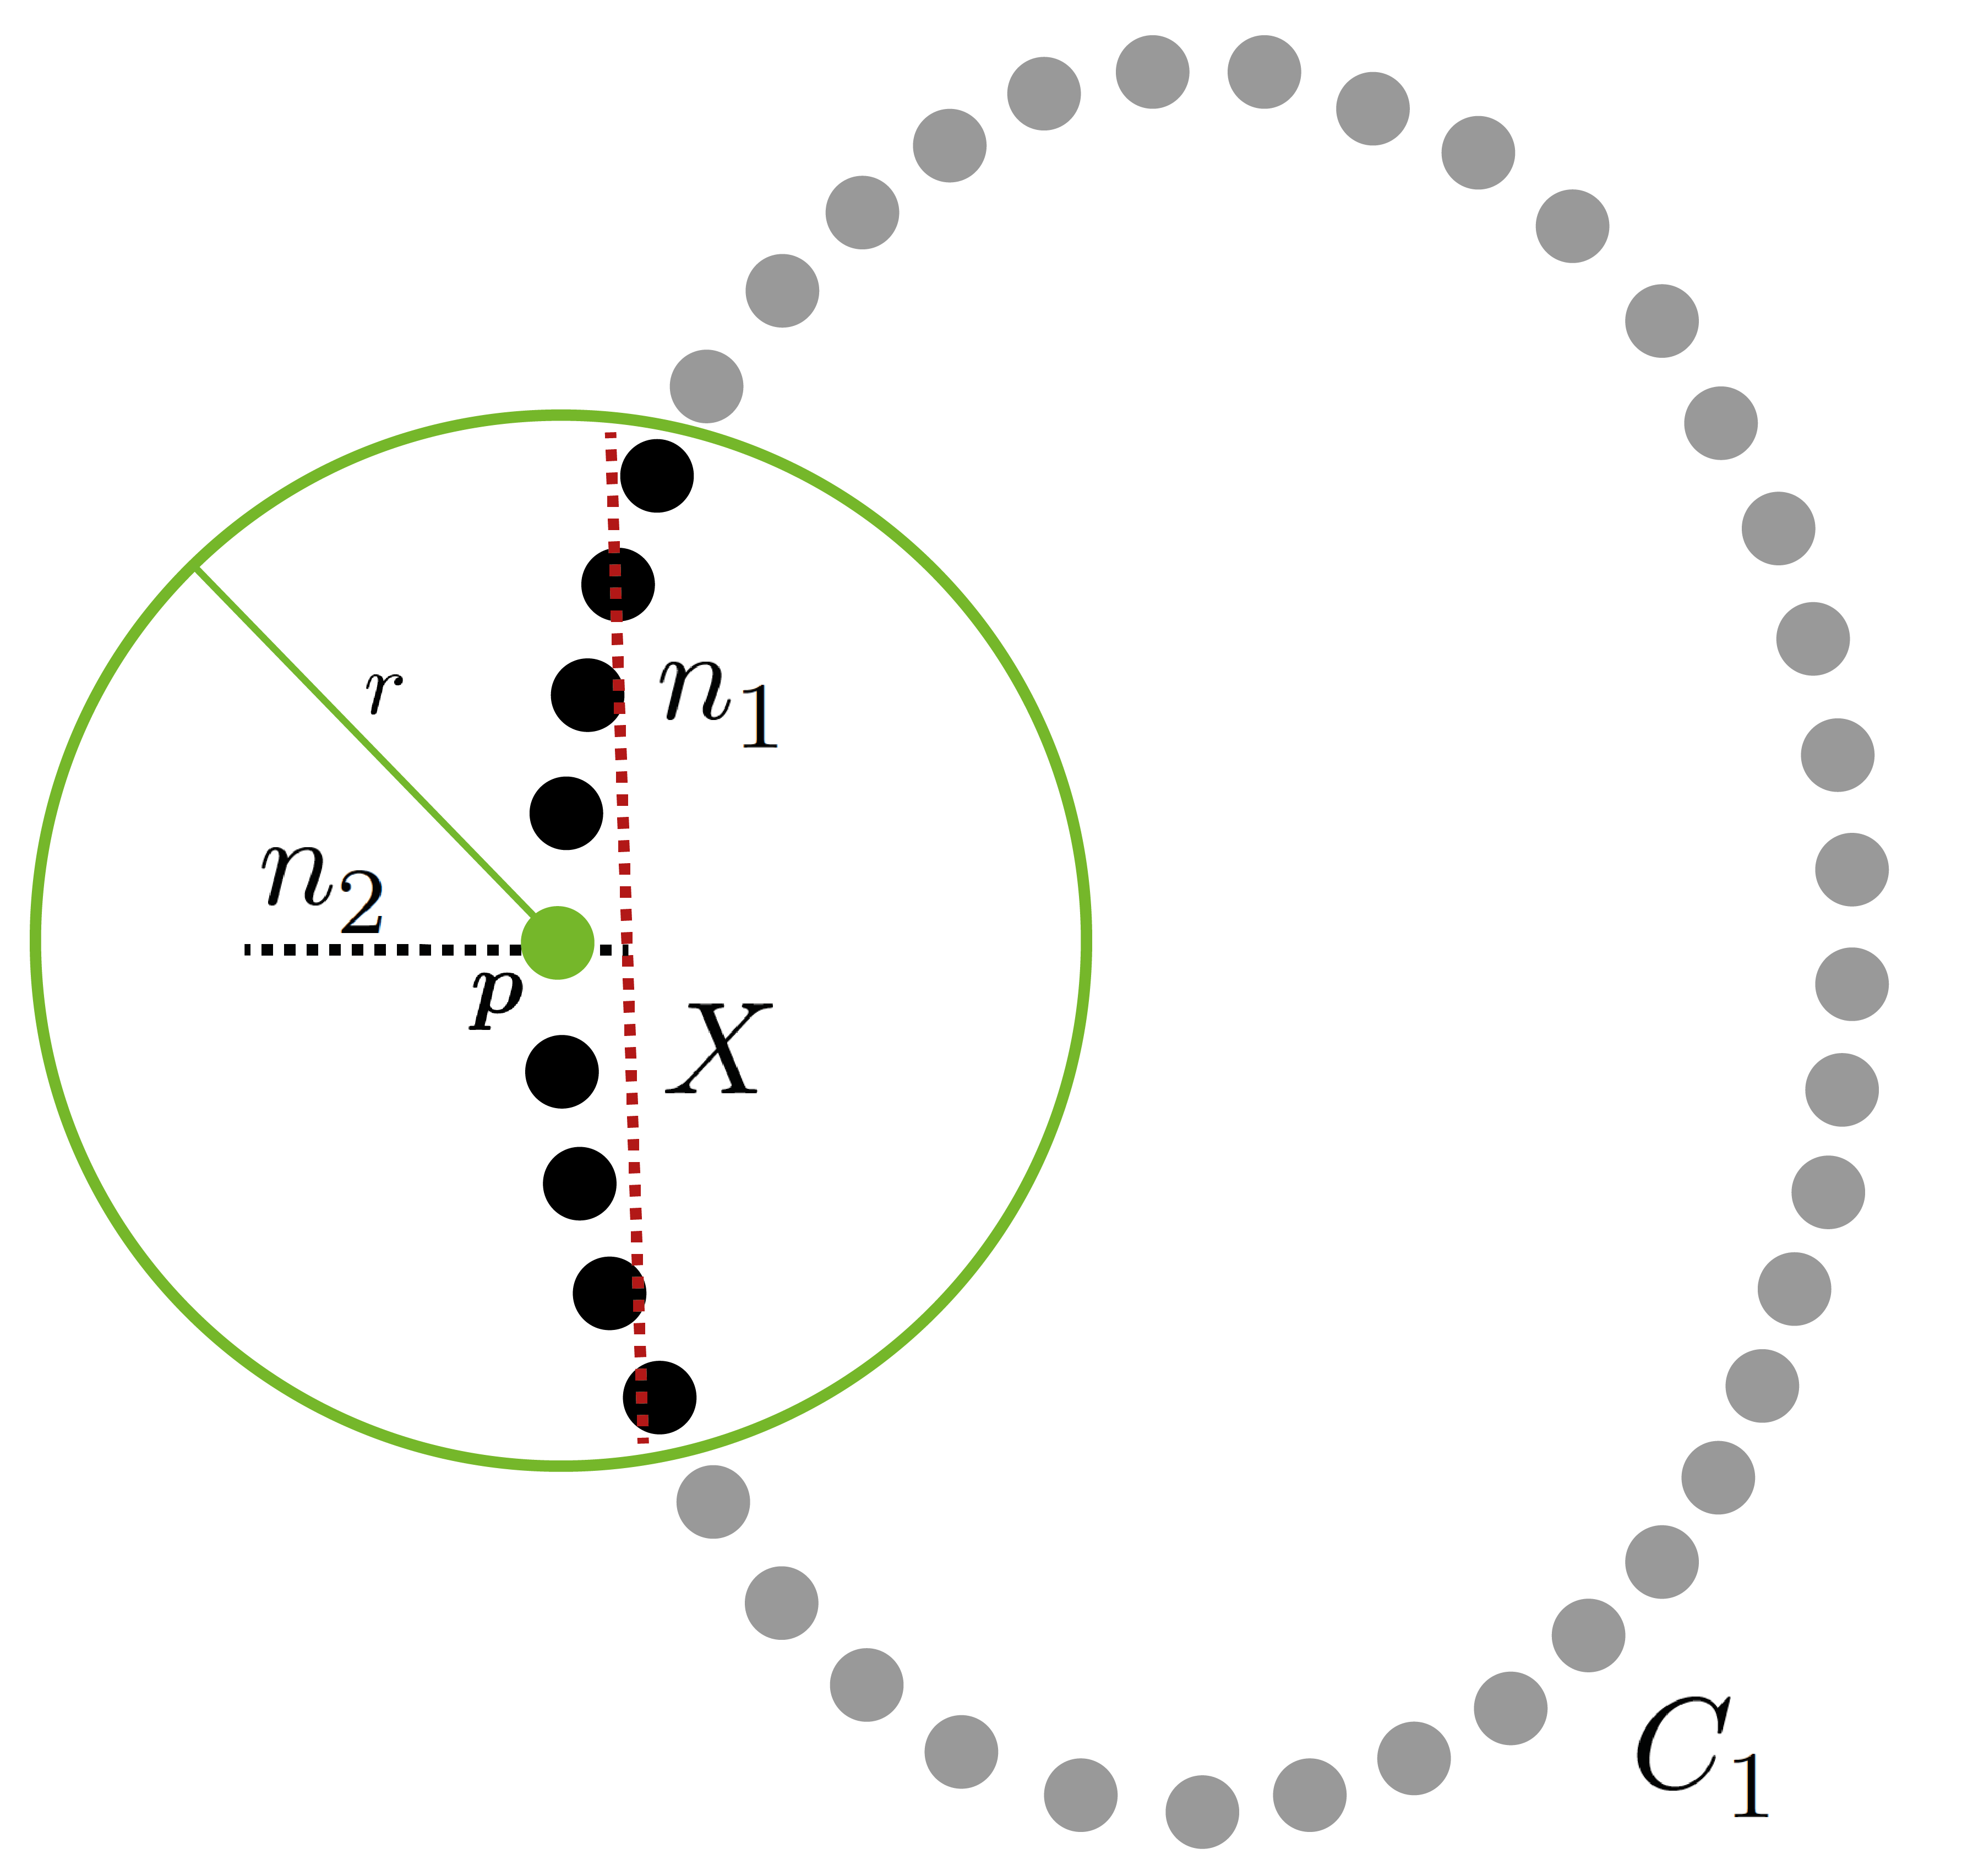
\includegraphics[width=0.4\linewidth]{normalEstimation}
	\caption{Normal estimation for a cluster point $\boldsymbol{p}$ of $C_i$ by a computation of the least squared fitting line $X$ of the neighborhood inside a radius $r$. Calculation of the eigenvectors $\vec{n_1}$ and $\vec{n_2}$ by the covariance matrix of all $k$ points.}
	\label{fig:normalEstimation}
\end{figure}
%%
As a next step, it is required that all normals are equally oriented. Basically, all $n$ computed normals are traversed globally, starting with a normal $\vec{n_i}$ of a point $p_i$. Thereby, it is of particular importance to select a normal that assures consistent orientations between $C_1$ and $C_2$. Taking its orientation as parent normal $\vec{n_p}$, the angle $\delta$ between $\vec{n_p}$ and all neighboring normals $\vec{n_k}$ 
%%
\begin{equation}
\delta = \vec{n_p} \cdot \vec{n_k}, \quad \text{for $|\vec{n_p}|, |\vec{n_k}| = 1$}
\end{equation}
%%
is computed. In case of $\delta < 0$, $\vec{n_k}$ requires to be flipped 180° ($\vec{n_k} = -\vec{n_k})$. If all $k$ normals have been verified to be oriented in consideration of $\vec{n_p}$ any $\vec{n_k}$ is selected as current $\vec{n_p}$. The whole algorithm proceeds until all $n$ normals have been verified to correspond with their parent normal $n_p$. Results of the normal flipping procedure can be seen on figure XX.

%TODO: Picture of normal estimation + flipping

\subsection{SPFH and FPFH}

The simplified point feature histogram (SPFH) for a point $\boldsymbol{p}$ is then computed by using three geometric features. Between $\boldsymbol{p}$ and each of its $k$ neighbors $\boldsymbol{p_k}$ given a threshold $\tau$, those features are computed -- $\boldsymbol{p_i}$ is thereby the point having the smaller angle between its normal and the line connecting the point set, $\boldsymbol{p_j}$ corresponds to the remaining point. Using their normals $n_i$ and $n_j$ a Darboux $uvn$ frame $(u = n_i, v = (p_j - p_i) \times u, w = u \times v)$ is computed. The following angles
%%
\begin{equation}
\begin{split}
\alpha = v \cdot n_j
\\
\phi = (u \cdot (p_j - p_i))/\|p_j - p_j\|
\\
\theta = arctan(w \cdot n_j, u \cdot n_j)
\end{split}
\label{eq:AngularVariations}
\end{equation}
%%
are computed. In a second step for each point $\boldsymbol{p_i}$ again all $n$ neighbor points given a threshold $\tau$ are computed. The simple point histogram SPF of $p$ is then weighted to the final histogram
%%
\begin{equation}
FPFH(\boldsymbol{p}) = SPF(\boldsymbol{p}) + \frac{1}{n} \cdot \displaystyle\sum_{i=1}^{n}\frac{1}{w_i} \cdot SPF(p_i)
\end{equation}
%%
where the weight $w_i$ represents the distance $d(\boldsymbol{p},\boldsymbol{p}_i)$. The influence region diagram for a Fast Point feature histogram for a query point $\boldsymbol{p_q}$ can be seen on Figure \ref{fig:FPFHregion}. 
%%
\begin{figure}[H]
	\centering
	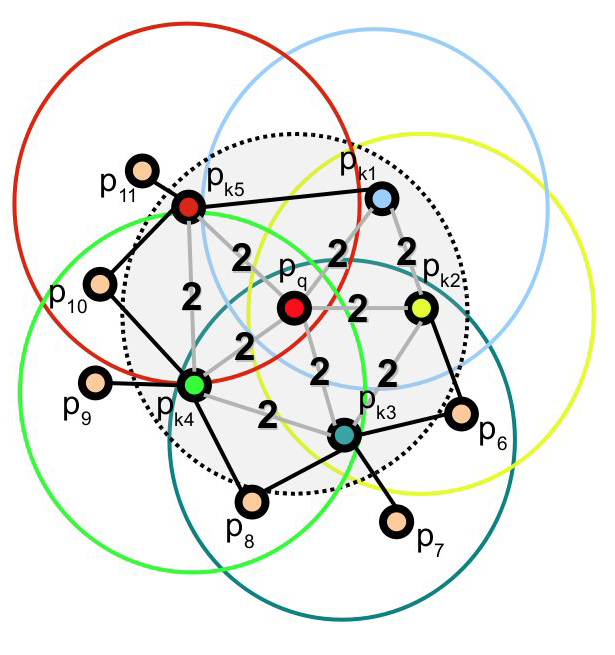
\includegraphics[width=0.4\linewidth]{FPFH_region}
	\caption{The point region for the calculation of the feature histogram for a query point $\boldsymbol{p}_q$. The histogram of $\boldsymbol{p}_q$ and its neighbors (inside the grey circle) is weighted with the further linked neighbors (colored circles) \cite{FPFH}.}
	\label{fig:FPFHregion}
\end{figure}
%%

\subsection{Feature histograms}
The resulting feature values in form of three angles between each two points are categorized using a histogram with $q^f$ bins to consider all possible combinations of the feature values. Thereby, $q$ represents the number of intervals and $f$ the number of feature values, in this case 3. After the allocation the associated bin at the index $idx$
%%
\begin{equation}
idx = \displaystyle\sum_{i=1}^{i \leq f}q(f_i) \cdot 2^{i-1}
\end{equation}
%%
is incremented by 1. The function $q(f)$ returns the interval the feature is allocated to, ranging from 0 to $q - 1$. Finally, each bin contains the number of point pairs that are allocated in the specified value interval.As soon as the feature histograms of all points from $C_1$ and $C_2$ are computed only salient histograms are taken as comparison for point correspondence between $C_1$ and $C_2$. This can be done with a normal distribution over all histograms $h$ to reject histograms being similar to the mass. As a histogram with $q^f$ bins might contain a lot of zero values, each feature can be allocated to its own histogram, resulting in $f$ histograms with $q$ bins.

\subsection{Adaptions for 2D}
In order to compute those 3D features for 2D points, those can be treaded like 3D points by setting each z-coordinate to 0, by doing so, all calculations can be conducted straight forward. However, one feature would be redundant, as $v$ is the same vector for each point. No considerable deductions could be detected. 

%TODO: what has been changed in 2D?

\section{Initial alignment: Largest rigid part}
\label{LRP}

As opposed to the linear approach by subdividing $C_1$ and $C_2$ into sub clusters, the feature-based approach is implemented to detect as an initial step the largest rigid part (LRP) of $C_1$ and $C_2$. Proceeding from there, all other linked parts are detected by region growing and reapplying the algorithm. This approach has been originally implemented for 3D point clouds by Mitra \cite{Mitra07}.

\subsection{Basic functionality}
\label{functionalityLRP}
As an initial step, the LRP algorithm  attempts to detect the most reliable correspondences between $C_1$ and $C_2$. For that, local descriptors (see section \ref{FPFH}) are computed. The requirement for a sparse correspondence between two cluster points $\boldsymbol{p}_i(x,y)$ and $\boldsymbol{p}_j(x,y)$ is that they are \textit{reciprocal}, which means that the according point feature histograms are the most similar from each other. Some of the sparse correspondences are assumed to be wrong. Therefore, by applying RANSAC to the point correspondences, a single rigid transformation is aimed for to detect the so-called ``largest rigid part'' (LRP), which is supported by the largest corresponding point cluster between $C_1$ and $C_2$. In case of a human, this would be the torso. Subsequently, all linked rigid parts to the LRP are detected by recursively applying the algorithm on grown clusters from the current LRP.

\subsection{Implementation steps}

In order to re-implement the algorithm in 2D, only small modifications concerning point coordinates had to be accomplished. The most crucial part of the whole algorithm is the initial alignment of $C_1$ and $C_2$ in order to detect the actual largest rigid part of the articulated object. This step is of particular importance, as the subsequent detection of further rigid parts proceeds from there. Therefore, as first step, sparse correspondences between $C_1$ and $C_2$ have to be detected (see subsection \ref{correspondences}). The initial idea was to detect correspondences by applying the ICP only proceeding the iterative transformation calculation with the most reliable correspondences. However, this approach did not manage to detect the desired correspondences of the largest rigid part (see section \ref{ResultsLRP}).

\begin{enumerate}
	\item The PCA is employed on the input clusters $C_1$ and $C_2$ to estimate the normals of all points.
	\item Point feature histograms (FPFH) are computed to detect sparse point correspondences between $C_1$ and $C_2$. A Point correspondence between $C_1$ and $C_2$ needs to be \textit{reciprocal}.
	\item The RANSAC approach is applied on those correspondences to detect a $T_j$ that rejects wrong point correspondences. Clusters are detected from all corresponding points by applying region growing.
	\item The LRP is assigned to the resulting biggest point cluster.
	\item Proceeding with the LRP, unmatched clusters to $C_1$ and $C_2$ are seeked by region growing from the LRP. The algorithm is then reapplied on those clusters until all rigid parts have been discovered.
\end{enumerate}

\subsection{Detection of sparse correspondences}
\label{correspondences}

As a first step, the 2D hulls of an articulated object in two different poses are taken as input (see Figure XX). Subsequently, the feature histogram for each point of $C_1$ and $C_2$ (see section \ref{FPFH}) is computed. For the detection of sparse correspondences the feature histograms are compared by means of normal distribution, mean and peak. The most similar histograms are selected as correspondence if they are \textit{reciprocal}.
As some of those correspondences might be wrong (see figure XX), a RANSAC approach is applied on all correspondences to reject false ones (see subsection \ref{detectionLRP}).

%TODO: add articulated puppet in two poses for input PICTURE

%TODO: image of histograms + most unique feature points

\subsection{Detection of the largest rigid part}
\label{detectionLRP}
The dense point correspondences from the previous computation step (see subsection \ref{correspondences}) may contain several errors. Therefore, RANSAC is applied as a next step to detect a single rigid transformation $T$ that leads to the biggest overlapping point cluster of $C_i$ and $C_j$. Thereby, in each iteration, 3 random correspondences are selected and used for the calculation of $T$ which is applied on $C_i$ to be translated on $C_j$. Subsequently, clusters are grown from all corresponding points with an euclidean distance $d(\boldsymbol{p}_i,\boldsymbol{p}_j)$ again below a predefined threshold $\tau$. The procedure is applied both on $C_i$ and $C_j$ which results in two rigid parts as output. In case of symmetric poses, the RANSAC would not be required, as the largest rigid part (the torso) would be almost perfectly aligned and taken as input for the region growing. But still, to cover as many cases as possible, this computation step is necessary. 

\subsection{Cluster detection by region growing}
\label{cluster}
After successfully detecting a ``largest rigid part'' $P_i$ and $P_j$ for each input clusters $C_i$ and $C_j$ they are added to a list of rigid parts $\mathcal{P}$. Potential linked rigid parts are detected from region growing of all unclustered points $\mathcal{U} =  \{\boldsymbol{u}_1,\ldots,\boldsymbol{u}_n\}$. Those comprise all cluster points of $C_1$ and $C_2$ excluding already detected largest rigid parts $\mathcal{P}$. The region growing initiates with the first point $\boldsymbol{u}_1$ of the unclustered points $\mathcal{U}$ to form a cluster $C_i$. Another point of the unclustered points $\boldsymbol{u}_j$ is added to $C_i$, if the euclidean distance $d(\boldsymbol{p}_i,\boldsymbol{u}_j)$ to any point in $C_i$ is below the threshold $\tau$. If no further unclustered points can be added, the region growing initiates again with the first unclustered point $\boldsymbol{u}_1$ that has not been added by region growing until all points traversed the procedure. The result is a set of clusters $\mathcal{C}$ for each $C_i$ and $C_j$. Subsequently, a preliminary joint $\boldsymbol{j}_i$ for each output clusters is stored, by detecting the two nearest points of $C_i$ and $P_i$. The joints are required for following cluster correspondence and joint weights for the ICP (see subsection \ref{CorrespondingClusters} and \ref{JointWeights}).

\subsection{Establishment of corresponding clusters}
\label{CorrespondingClusters}
In case of detecting more than one cluster for each $C_i$ and $C_j$, which might be for example the case for the extremities linked to the torso, it must be verified which clusters correspond to each other. This step is essential, as the algorithm is called recursively (starting from \ref{correspondences}) with two new input clusters. Thereby, the provisional joints $\boldsymbol{j}_i$ are used to associate two clusters of $C_i$ and $C_j$ by detecting the closest joint with the euclidean distance $d(\boldsymbol{j}_i,\boldsymbol{j}_j)$.

\subsection{Joint weights}
\label{JointWeights}
In order to iteratively detect largest rigid parts that are actually linked to another detected ``largest rigid part'', the preliminary joints resulting from \ref{cluster} are used as weights. Thereby, points being located far away from joints, do not contribute as much to the matching error as point located near a joint. By doing so, joint consistency across two poses is enforced. As an alternative to the ICP clusters with calculated joints only need to be rotated around them. As a result, a matching error $e$ 
%
\begin{equation}
	e = \displaystyle\sum_{i=1}^{m}\| \boldsymbol{p}_i - \boldsymbol{q}_i\|^2 \cdot \| \boldsymbol{p}_i - \boldsymbol{j}_i\|
\end{equation}
%
is achieved which combines the distance to the closest point and to the cluster's joint. Thereby, not only successful correspondences are taken as input but all points, that the error is expressive. The final correspondence equals to the rotation around the joint $\boldsymbol{j}_i$ with the smallest error $e$. 

\section{Implementation}
\label{ImplementationLRP}
The individual steps of the largest rigid part algorithm have also been split in the implementation for better overview. 
%
%TODO: Add code snippets to implementation LRP
%
\subsection{ICP}
One main part of the algorithm is the modified implementation of the ICP using Procrustes fitting to compute a transformation that detects sparse point correspondences. Thereby, only reciprocal correspondences within a specific distance $\tau$ contribute to the calculation. The final point correspondences of $C_i$ and $C_j$ are stored in a \texttt{Map<Integer, Integer>} containing the indices of the corresponding points. This is because the storage of points in the form $\boldsymbol{p}_i(x,y)$ would underly a specific transformation, which is applied during the ICP and initial alignment. For further computations using the RANSAC, no transformations are desired. As the main difficulty is the right initial alignment of the actual largest rigid part (torso) the value of the distance threshold $\tau$ is chosen generously. As a result, a higher number of false point correspondences is detected which has to be compensated by RANSAC (see subsection \ref{RANSAC}).

\begin{lstlisting}
...
for (Map.Entry<Integer, Integer> entry : reference.entrySet()) {
Integer referenceIndex = entry.getKey();
Integer targetIndex = entry.getValue();

	if (target.containsKey(targetIndex) && target.get(targetIndex) == referenceIndex) {
		referencePoints.add(originalReference.get(referenceIndex));
		targetPoints.add(originalTarget.get(targetIndex));
		finalAssociations.put(referenceIndex, targetIndex);
	}
}
...
\end{lstlisting}

\subsection{Image Features}
%
%TODO: implementation of features (incl normals)
%
As a first step, the normals of all points $n$ of $C_1$ and $C_2$ are computed. For this matter a class was developed that takes a point $p_i$ with its $k$ neighbors as input. Then, the least fitting error line is detected (as described in section \ref{correspondences}) and the eigenvector being associated with $\lambda_2$ is selected as normal vector $\vec{n}$ for $p_i$. 
The computation of the least fitting line can be seen on figure XX.
%%
%TODO: least fitting line PICTURE 
%%
An essential part of the normal estimation is the right orientation of all normals, which can be seen on figure XX.
%%
%TODO: normal orientation PICTURE
%%
Subsequently, the FPFH features are computed. For that, again a point $p_i$ is selected with its $k$ neighbors an taken as input. A \texttt{ClusterPoint} was implemented to store the normal $n_i$ for each point and the feature histogram in form of an \texttt{int[]} array. The \texttt{FPFH} class implements various operations for vectors, like a dot or cross product. For the comparison of two histograms from $C_1$ and $C_2$ a gaussian distribution was computed on all histograms to only remain unique histograms for further comparisons. Unique and reciprocal point correspondences between $C_1$ and $C_2$ \texttt{Map<Integer,Integer>} are returned  in form of their indices.

%TODO: add code snippet of feature calculation
%TODO: add resulting histograms of unique points + normal distribution PICTURE

\subsection{RANSAC}
\label{RANSAC}
The RANSAC algorithm takes the computed dense correspondences between $C_i$ and $C_j$ in form of a \texttt{Map<Integer, Integer>} as input. As a first step, three random correspondences are selected from the map to calculate an affine transformation between the three resulting points from each $C_i$ and $C_j$. The initial orientation and alignment is thereby irrelevant as the transformation $T$ is completely recalculated.

\begin{lstlisting}
public LargestRigidPart(Cluster c_i, Cluster c_j, Map<Integer, Integer> correspondences)
...
points1 = c_i.getPoints();
points2 = c_j.getPoints();
...
private void getRandomPoints(int num) {
	Integer[] keys = correspondances.keySet().toArray(new Integer[0]);
	Integer[] values = correspondances.values().toArray(new Integer[0]);

	for (int i = 0; i < num; i++) {
		index = (int) (Math.random() * correspondances.size());
		randomPoints1.add(points1.get(keys[index]));
		randomPoints2.add(points2.get(values[index]));
	}
}
...
\end{lstlisting}

Similar to the ICP, a closest point procedure with a threshold $\tau$ is conducted. The value is thereby considerably smaller than in the ICP as a right alignment during any iteration is assumed. Unlikely the ICP, no error during the Procrustes fit is accumulated, instead the detected point correspondences are taken as input in the region growing \ref{RegionGrowing} procedure. The biggest cluster is stored and after all iterations returned as largest rigid part.

\subsection{Region growing}
\label{RegionGrowing}
The region growing algorithm is quite similar to the earlier described algorithm (see algorithm \ref{noiseRemoval}). There is also an adaptation, which does not only return the largest cluster, but all clusters above a certain size. The detected clusters are handled in a \texttt{Stack<Cluster>} in case of more than one detected clusters. Thereby, all clusters are pushed on the stack. With each recursion two corresponding cluster $C_i$ and $C_j$ are popped from the stack and taken as input for the whole algorithm. If again more clusters are detected they are pushed on the stack and treated before recently added clusters.

\section{Results}
\label{ResultsLRP}

As the input point cloud of an articulated object is in 2D, the imitation of the object's hull is required. As a consequence, the region growing is much more error-prone, as unlikely in 3D, the points of a rigid part have a considerable lower number of neighbors. In case of a few missing cluster points from a rigid part, it will not be fully detected during the region growing due to the gaps. To counteract this behavior, joints are added to each rigid part, that more links for region growing are available. 

%TODO: add pictures of LRP results

The first main difficulty is the first alignment of the two input clusters $C_1$ and $C_2$. As the execution of the algorithm is only dependent on a succesful alignment, for test cases the assumption was made, that the orientation of the two poses are initially right. The main drawback of the ICP was that the starting position of the two main clusters $C_1$ and $C_2$ had to be ideal that the largest rigid part could be detected. However, this could not be guaranteed as asymmetrical body poses would influence the orientation (see Figure XXX) of the whole cluster $C_1$. As a result, reciprocal point correspondences could not be detected that would lead to the largest rigid part.

\subsection{Main drawbacks}
The main drawback of the algorithm represents the first initial alignment of the two poses of the articulated object. Thereby, it is directly dependent on the symmetry of the pose. The less symmetry the higher the changes that the initial alignment on the largest rigid part might fail. The reason is that the ICP expects a good starting alignment. As it is assumed that the major largest rigid part contributes most to the principal axis and the initial alignment, it would work. But in case of an unbalance of the linked parts, the alignment of the LRP might shift in a certain direction and it might not be detected during the ICP. As a result the whole algorithm fails. Furthermore, touching of rigid parts (e.g. the hand touches the leg) constitute difficulties as the region growing would not detect those as potential linked clusters. 

\section{3D implementation}

The next step would be to implement the approach in 3D. A similar implementation was done by Mitra \cite{Mitra07} (see section \ref{functionalityLRP}) by using the PCL. Most essential functions like FPFH and subsampling for large point clusters are already provided. A good dataset would be thereby the SCAPE, which offers different poses of a scanned human. 

%TODO: Write what fails/main problems/solutions







